\documentclass{amu_these}

\begin{document}

%\cfoot{pagenumber}
%\rhead[]{}
%\clearscrheadfoot
\chead{}

% générer la page de titre
\titlepage
\titlepage

\usefont{T1}{qhv}{m}{n}\selectfont{} %sans sérif page de titre

\vspace*{-2cm}
\begin{center}
	\begin{minipage}[c]{0.25\linewidth}
		\raggedright 
\includegraphics[height=50px]{logo_amu}
	\end{minipage}\hfill
	\begin{minipage}[c]{0.25\linewidth}
		\raggedleft 
\includegraphics[height=50px]{wikimedia_fr_logo}
	\end{minipage}\hfill 
\end{center}

\begin{flushleft}
        \vspace{0.2cm}
    \LARGE UNIVERSITE D’AIX-MARSEILLE\\
        \vspace{0.2cm}
    \Large ECOLE DOCTORALE\\
        \vspace{0.2cm}
    \normalsize FACULTE\\
        \vspace{0.2cm}
    LABORATOIRE\\
    \begin{center}
        \vspace{2cm}
    THESE DE DOCTORAT\\
    \end{center}
        \vspace{0.5cm}
    Discipline :\\
    Spécialité :\\
    \begin{center}
        \vspace{0.5cm}
    \Large Prénom NOM\\
        \vspace{1cm}
    \large Titre de la thèse : sous-titre\\
    \end{center}
        \vspace{3cm}
    \normalsize Soutenue le 01 janvier 2012\\
        \vspace{0.4cm}
    Composition du jury :\\
\end{flushleft}

\vspace{0.4cm}

\begin{tabular}{lll}
Prénom NOM & Affiliation & Président du Jury \\
    \vspace{0.08cm}
Prénom NOM & Affiliation & Rapporteur \\
    \vspace{0.08cm}
Prénom NOM & Affiliation & Rapporteur \\
    \vspace{0.08cm}
Prénom NOM & Affiliation & Examinateur \\
    \vspace{0.08cm}
Prénom NOM & Affiliation & Examinateur \\
    \vspace{0.08cm}
Prénom NOM & Affiliation & Directeur de thèse \\
\end{tabular}

\usefont{T1}{bch}{m}{n}\selectfont{} % sérif corps du texte

\newpage
\thispagestyle{empty}
\null

\newpage
\chapter*{Résumé}
\lipsum[1]

\vspace{0.5cm}
Mots clés : géométrie algorithmique, complexe planaire et rectangulaire, géodésique, courbure globale non-positive
\addcontentsline{toc}{chapter}{Résumé}

\newpage
\chapter*{Abstract}
\selectlanguage{english}
\lipsum[1]\index{Lorem ipsum}

\vspace{0.5cm}
Keywords: computational geometry, planar and rectangular complex, geodesic, global nonpositive curvature
\selectlanguage{french}

\addcontentsline{toc}{chapter}{Abstract}

\newpage
\tocloftpagestyle{plain}
\tableofcontents

\newpage
\tocloftpagestyle{plain}
\listoffigures
\addcontentsline{toc}{chapter}{Table des figures}

\newpage
\chapter*{Introduction}
\lipsum[1-2]
\addcontentsline{toc}{chapter}{Introduction}

\newpage
\chapter{Première partie}
\section{Généralités sur la fusion thermonucléaire}
Lors d'une réaction de fusion, deux noyaux légers s'assemblent pour former un noyau plus lourd. Pour obtenir une réaction de fusion, il faut rapprocher suffisamment deux noyaux qui, puisqu'ils sont tous deux chargés positivement, se repoussent. Une certaine énergie est donc indispensable pour franchir cette barrière et arriver dans la zone, très proche du noyau, où se manifeste l'interaction forte capable de l'emporter sur la répulsion électrostatique.
\\ %  retour à la ligne
La réaction de fusion la plus favorable est celle faisant intervenir le deutérium et le tritium: $$_{1}^{2}D^{+}~+~_{1}^{3}T^{+}~\rightarrow ~_{2}^{4}He^{2+}~(3,5\,\textrm{MeV})~+~n~(14,1\,\textrm{MeV}).$$
\noindent % pas d'indentation en début de paragraphe
\lipsum[1]\index{Lorem ipsum}
\section{Deuxième section de la première partie}
\lipsum[2]


\newpage
\chapter{Deuxième partie}
\section{Matériel et méthodes}
\subsection{Modèle animal}
\lipsum[1]
\subsection{Traitement expérimental}
\subsubsection{Hypergravité}
\label{hypergravite} % on peut mettre systématiquement un \label après chaque titre de partie au cas où un /ref{} serait nécessaire
L'hypergravité consiste à augmenter la force du vecteur gravitaire en lui sur-imposant la force centrifuge. En effet, la force centrifuge induite par la rotation se surimpose à la gravité terrestre ce qui permet d'avoir une force résultante dépendante de la vitesse de rotation. On utilise pour cela des centrifugeuses qui sont des carrousels équipés de nacelles suspendues à des axes libres permettant à la force résultante d'être perpendiculaire au plancher de la nacelle et ainsi obtenir une \og gravité \fg{} dont la force est supérieure à la gravité terrestre tout en maintenant, pour les individus expérimentaux, l'orientation \og naturelle \fg{} de celle-ci.
\lipsum[1-5]
Une première note de fin de document\endnote{Première note de fin de document.} et une seconde\endnote{Deuxième note de fin de document.} et ... \endnote{... note de fin de document.} \endnote{... note de fin de document.} \endnote{... note de fin de document.} \endnote{... note de fin de document.} \endnote{... note de fin de document.} \endnote{... note de fin de document.} \endnote{... note de fin de document.} \endnote{... note de fin de document.} \endnote{... note de fin de document.} Quisque ullamcorper placerat ipsum.\endnote{\lipsum[3]}.
\subsubsection{La centrifugeuse}
Les caractéristiques techniques de la \index{centrifugeuse} ont été décrites dans un article de \cite{jamon_ground-based_2008} et dans la partie \ref{hypergravite}. Brièvement, la centrifugeuse (Figure~\ref{photo_centrifugeuse}) est de grand diamètre (jusqu'à 3,6~m en rotation). Pour limiter les vibrations, la centrifugeuse repose sur des dispositifs anti-vibrations. Le bruit produit par la centrifugeuse est faible. A un mètre de distance, le niveau sonore n'est que de 58~dB contre 52~dB si la centrifugeuse est arrêtée. Les nacelles sont sur des axes libres et chacune peut contenir trois cages de type standard (364x206x131 mm) avec 4 souris par cage, soit un total de 48 souris. La centrifugeuse est équipée de caméras infra-rouge couplées à un système de vidéo-surveillance accessible sur internet. Cela nous permet de contrôler les niveaux d'eau et de nourriture ainsi que de conduire des études de l'activité des individus expérimentaux à distance, de jour comme de nuit. La quantité d'eau et de nourriture disponible par cage permet de faire fonctionner la centrifugeuse 3 semaines sans interruption. Les animaux ont à disposition 400~g de nourriture et 500~ml d'eau, mais la consommation de nourriture sur cette période est en moyenne de 209~g ($\pm$14), et la consommation d'eau de 258 ml ($\pm$21) pour une cage de 4 souris. 
\begin{figure}[h!tbp] % à voir
\vspace{0.5cm}
\setcapindent{2em}
  \centering
  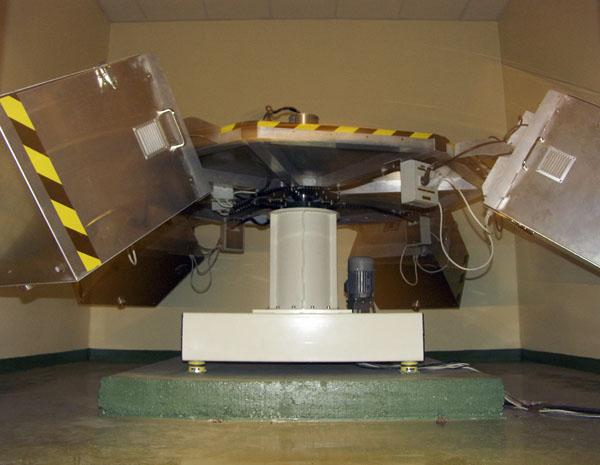
\includegraphics[width=0.7\textwidth]{photo_centrifugeuse}
  \caption[Photographie de la centrifugeuse]{Photographie de la centrifugeuse utilisée.}
  \label{photo_centrifugeuse}
\end{figure}
\lipsum[1]
\section{Deuxième section de la deuxième partie}
\lipsum[2]
\subsection{Première sous-section de la deuxième section de la deuxième partie}
\lipsum[4]
\subsection[Sous-sous-sous-partie 2]{Deuxième sous-section de la deuxième section de la deuxième partie} % entre [] pour affichage dans la TOC
\lipsum[4]Une note de bas de page\footnote{première note de bas de page} et une seconde\footnote{deuxième note de bas de page}.
\subsubsection{Ce titre de section ne s'affiche pas dans la TOC : tocdepth=2}
Nam dui ligula, fringilla a, euismod sodales, sollicitudin vel, wisi \parencite{zohdy_mapping_2012}. \lipsum[3] % citation entre parenthèses et tous les auteurs
\paragraph{Ce titre de section n'est pas numéroté : secnumdepth=3}~~\\ % "~~\\" fait le saut de ligne après le titre de 'paragraph'

% ce saut de ligne dans le code indente 'paragraph'
\lipsum[3]


\newpage
\chapter{Troisième partie}
Voir (Tableaux~\ref{table:alpha}~et~\ref{table:multi}).
\lipsum[3]
\begin{table}[h!tbp]
\begin{center}
\begin{tabular}{|c | c | c |}
\hline
$\lambda$ (nm) & $(\alpha_{\lambda}/\alpha_{426,7})_{moy}$ & écart type \\
\hline
391,9 \& 392,1 & 0,12 & 0,01 \\
588,9 \& 589,2 & 0,45 & 0,07 \\
657,8 \& 658,3 & 6,70 & 0,06 \\
711,3 & 0,16 & 0,01 \\
711,6 & 0,15 & 0,01 \\
712 & 0,31 & 0,02 \\
\hline
\end{tabular}
\end{center}
\caption[Valeur moyenne et écart type des rapports $\alpha_{\lambda}/\alpha_{426,7}$]{Valeur moyenne et écart type des rapports $\alpha_{\lambda}/\alpha_{426,7}$ mesurés pour les chocs plasma de la deuxième série.}
\label{table:alpha}
\end{table}

\lipsum[2]

Ajout d'une nouvelle entrée d'index de la centrifugeuse\index{centrifugeuse}.


\newpage
\chapter*{Conclusion}
\chapter*{Conclusion}
\addcontentsline{toc}{chapter}{Conclusion}
\lipsum[1-2]
\addcontentsline{toc}{chapter}{Conclusion}

\newpage
%\printbibliography
\addcontentsline{toc}{chapter}{Bibliographie}

\end{document}
